%% This is an example first chapter.  You should put chapter/appendix that you
%% write into a separate file, and add a line \include{yourfilename} to
%% main.tex, where `yourfilename.tex' is the name of the chapter/appendix file.
%% You can process specific files by typing their names in at the 
%% \files=
%% prompt when you run the file main.tex through LaTeX.

\chapter{Whole-genome sequencing identifies emergence of a quinolone resistance mutation in a case of \emph{Stenotrophomonas maltophilia} bacteremia}
\label{chap:steno}

\begin{quote}
\emph{In this chapter we use next-generation sequencing to reveal the mechanism of emerging drug resistance in a case of hospital-acquired infection following the failure of routine antimicrobial therapy. Whole genome sequences for \emph{Stenotrophomonas maltophilia} serial isolates from a bacteremic patient before and after development of levofloxacin resistance were assembled \emph{de novo} and differed by one single-nucleotide variant in \emph{smeT}, a repressor for multidrug efflux operon \emph{smeDEF}. Along with sequenced isolates from five contemporaneous cases, they displayed considerable diversity compared against all previously published complete genomes. Whole genome sequencing and complete assembly can conclusively identify resistance mechanisms emerging in \emph{S. maltophilia} strains during clinical therapy.}
\end{quote}

\section{Introduction}

\emph{Stenotrophomonas maltophilia} is an aerobic, non-fermenting, and motile Gram-negative bacterium that is increasingly recognized as a cause of hospital-acquired infections with crude mortality rates of 14–69\% in cases of bacteremia.\autocite{Brooke2012} Treatment of \emph{S. maltophilia} infections is challenging due to the pathogen’s intrinsic resistance to many antibiotic classes via drug efflux pumps, beta-lactamase production, and decreased membrane permeability.\autocite{Brooke2012} Resistance phenotypes are known to change during the course of treatment, which complicates interpretation of automated drug susceptibility testing (DST) results.\autocite{Garrison1996} A mutant strain of \emph{S. maltophilia} with emerging resistance to tetracycline, chloramphenicol, and quinolones was previously characterized following in vitro tetracycline selection.\autocite{Alonso1997,Sanchez2002} However, little is known about the genetic and molecular mechanisms underlying acquired resistance in the clinical setting—particularly for quinolones, where in contrast to other Gram-negatives, the quinolone-resistance determining region (QRDR) of topoisomerase genes is often unaltered.\autocite{Valdezate2005} In this report, we describe the first reported use of whole genome sequencing (WGS) in serial clinical isolates to definitively identify an acquired quinolone resistance mutation in \emph{S. maltophilia}. WGS was performed for the initial and subsequent \emph{S. maltophilia} blood culture isolates from a patient where acquired quinolone resistance was observed (Patient 1) and five other patients (Patients 2-6) selected from a two-month period in 2013 at The Mount Sinai Hospital. 

\section{Case report}

Patient 1 was a 56 year-old man with a history of pancreatic cancer and a Whipple procedure eleven years earlier who presented to The Mount Sinai Hospital with variceal bleeding at the hepaticojejunostomy site. A transjugular intrahepatic portosystemic shunt was placed, which was complicated by thrombosis. In the following weeks, he had several episodes of polymicrobial bacteremia and was treated with multiple courses of antimicrobials, including a 10-day course of levofloxacin. Two months after levofloxacin exposure, he developed another episode of polymicrobial bacteremia. Blood cultures intermittently grew \emph{S. maltophilia}, \emph{E. faecium}, and \emph{Candida parapsilosis} despite appropriate antimicrobial therapy. Automated DST showed that the first \emph{S. maltophilia} isolate acquired was susceptible to levofloxacin (minimum inhibitory concentration [MIC] 0.5µg/mL) and trimethoprim/sulfamethoxazole (TMP-SMX; MIC ≤20 µg/mL). He was treated with 400 mg intravenous ciprofloxacin every 8 hours, but blood cultures nine days later again grew \emph{S. maltophilia}, now resistant to levofloxacin (MIC >32µg/mL) while still susceptible to TMP-SMX (MIC 1µg/mL). Ciprofloxacin therapy was stopped and intravenous TMP-SMX was given every 8 hours; subsequent cultures did not grow \emph{S. maltophilia}.

\section{Methods}

Standard culturing and susceptibility testing for levofloxacin and SXT were performed by automated microbroth dilution with Vitek2® (bioMérieux). Antimicrobial sensitivities were reported and interpreted according to the 2015 CLSI guidelines for \emph{S. maltophilia}.\autocite{ClinicalandLaboratoryStandardsInstitute2015} Isolates were then stocked and frozen at -80°C. Levofloxacin and SXT susceptibilities for all isolates in this study were later confirmed by Etest (bioMérieux) at 24 hours. To prepare for sequencing, isolates were grown from single colonies in tryptic soy broth, and DNA extraction was performed as previously described.\autocite{Altman2014}

\subsection{Genome sequencing}

Sequencing was performed to a depth of coverage of >150x per genome using the P4-C2 sequencing enzyme and chemistry at the manufacturer’s specifications on the PacBio RSII platform (Pacific Biosciences, Menlo Park, CA). For ISMMS2 and ISMMS2R, Sanger sequencing was additionally performed on six PCR-amplified regions encompassing the one single nucleotide variant (SNV) and five one-base indels that differentiated the two PacBio assemblies. Conventional PCR amplification was performed with Choice-Taq Blue (Denville Scientific) and included an initial denaturation step of 180s at 95°C, 30 cycles of denaturation, annealing, and extension at 95°C/30s, 60°C/30s, and 72°C/30s respectively, and a final extension step of 300s at 72°C. Primer sequences are as follows: for the SNV, \texttt{5’-CAAGGTGCTGACCGAAATGC-3’} forward and \texttt{5’-ACACGCCATCCTTCACGTAG-3’} reverse; and for the five indels, \texttt{5’-GCATGGAAGTACCACTGGGT-3’} forward + \texttt{5’-TTGGAGGGGTGGTAAAACGG-3’} reverse, \texttt{5’-TGGCCAACCCCTTCTATGTC-3’} forward + \texttt{5’-CCATGGCCACAGCAAAATGG-3’} reverse, \texttt{5’-CTGCCTTCGGTCACTTCGT-3’} forward + \texttt{5’-TGGAAGTCTCGCTGGAAGGT-3’} reverse, \texttt{5’-GCCCTCTACACCGTCTTTCC-3’} forward + \texttt{5’-GAACTACCGGACGGCTTTGA-3’} reverse, and \texttt{5’-AACTTCTTCGTGTCGGTCCC-3’} forward + \texttt{5’-AGAACTACCGGACGGCTTTG-3’} reverse. Sequences on both strands of the amplified products were determined at an external sequencing facility (Macrogen Inc., Rockville, MD) using the standard Sanger dideoxy-terminator method and the same primers.

\subsection{Sequence assembly and annotation}

Sequencing data was processed and assembled de novo using PacBio’s Hierarchical Genome Assembly Process\autocite{Chin2013} (HGAP, version 3) in the SMRTanalysis toolkit (version 2.3.0) using standard pre-assembly pipeline parameters. Custom scripts were used to circularize the draft assemblies and orient them similarly to reference assemblies K279a, R551-3, D457, and JV3 using the \emph{gyrB} locus as a landmark; these scripts are available at \url{https://github.com/powerpak/pathogendb-pipeline/releases/tag/steno\_v1.0} (\textsc{doi}:\href{http://dx.doi.org/10.5281/zenodo.17295}{10.5281/zenodo.17295}) within the files \texttt{scripts/circularizeContigs.pl} and \texttt{scripts/fasta-orient-to-landmark.pl}. To eliminate overhanging sequence at the end of contigs and to increase accuracy, raw reads were re-mapped to the circularized assemblies using Blasr and the final consensus was re-called using Quiver. Initial annotations were created using the RAST server\autocite{Overbeek2014} with specific annotation of sme genes derived from BLAST queries.
Depth of coverage reported in Table 1 was calculated by SMRTanalysis (version 2.3.0) during re-mapping of reads to the circularized draft assembly.

\subsection{Accession numbers}

Sequences and annotations for reference assemblies of clinical \emph{S. maltophilia} isolates K279a, R551-3, D457, and JV3 were obtained from GenBank/RefSeq at accession numbers \texttt{AM743169.1}, \texttt{NC\_011071.1}, \texttt{NC\_017671.1}, and \texttt{NC\_015947.1}, respectively. These represent the entirety of assemblies for \emph{S. maltophilia} found in NCBI Assembly with an Assembly Level of “Complete Genome” (\url{http://www.ncbi.nlm.nih.gov/assembly/organism/40324/all/}) at the time of the study.\footnote{By 2017, excepting the three assemblies submitted as a result of this study, only one more complete genome (\href{https://www.ncbi.nlm.nih.gov/assembly/GCF\_002025605.1/}{ASM202560v1}) is available.} K279a and D457 were isolated from human infections, while R551-3 and JV3 were isolated from plants. Previously published sequences for the quinolone-resistance determining region (QRDR) of the \emph{gyrA}, \emph{gyrB}, \emph{parC} and \emph{parE} genes in \emph{S. maltophilia}\autocite{Valdezate2002} were obtained from EMBL/European Nucleotide Archive.

Complete genome sequences for ISMMS2, ISMMS2R, and ISMMS3 were deposited in GenBank at accession numbers \texttt{CP011305}, \texttt{CP011306}, and \texttt{CP011010}, respectively. Deposited sequences for ISMMS2 and ISMMS2R incorporate the Sanger corrected regions described above. Sequences for ISMMS4, ISMMS5, ISMMS6, and ISMMS7 were deposited as Whole Genome Shotgun projects at DDBJ/EMBL/GenBank under the accessions \texttt{JZIU00000000}, \texttt{JZIV00000000}, \texttt{JZIW00000000}, and \texttt{JZTX00000000}, respectively, with the versions described in this chapter at \texttt{JZIU01000000}, \texttt{JZIV01000000}, \texttt{JZIW01000000}, and \texttt{JZTX01000000}, respectively.

\subsection{Comparative genomic analysis}

Pairwise comparison between strains was performed with the MUMmer 3.23 package,\autocite{Delcher2003} firstly using nucmer for pairwise genome alignment. The resulting nucmer alignments were filtered for quality and uniqueness via the \texttt{delta-filter} tool (using the \texttt{–1} flag to identify top alignments between the reference and query intervals). To estimate phylogenetic tree distances, high-quality SNP and indel calls were assigned via the \texttt{show-SNPs} tool using the \texttt{–C} flag to only report SNPs in regions with unambiguous mappings. For ISMMS2 and ISMMS2R, \texttt{show-SNPs} was also used without the \texttt{–C} flag to verify that no additional SNPs or indels were in ambiguously mapped regions.

Mugsy version 2.2 was used to perform multiple sequence alignment of the whole genome sequences in order to find local collinear blocks (LCBs) of conserved sequence.\autocite{Angiuoli2011} These aligned blocks were used to establish a core genome (of 3.01 Mbp) across all isolates, from which a phylogenetic tree was constructed using RAxML version 8.0.2,\autocite{Stamatakis2014} employing the GTRGAMMA substitution model and performing 20 runs. Whole genome alignments for visualization of recombination events was performed with Mauve 2.4.0,\autocite{Darling2004} using the \emph{progressiveMauve} algorithm\autocite{Darling2010} with a minimum seed weight of 21, seed families enabled, and all other parameters at defaults. Clustal Omega\autocite{Sievers2011} was used for multiple sequence alignment of putative amino acid sequences, which were then rendered with ESPript version 3.0.\autocite{Robert2014}

\subsection{Epigenetic motif analysis}

For each isolate, initial DNA modification motifs were first predicted by a de novo motif discovery pipeline in SMRTportal (\texttt{RS\_Modifications\_Motif\_Analysis.1}). The pipeline searches for kinetic variations in DNA polymerization events recorded during sequencing that correlate with modifications in the template, with different modifications creating distinct kinetic profiles.\autocite{Clark2012,Fang2012} At the coverage depths reported for this study, the probability (power) of detecting a modification event at a site at the 0.1 significance threshold, if it is truly modified, exceeds 99.99\%.\autocite{Fang2012} Raw predictions, which often have incorrectly- or over-called motifs, were further refined by a re-analysis of the raw data using a single molecule level characterization method.\autocite{Beaulaurier2015} Conceptually, this method was used to check the single molecule level methylation status of each putative motif and its neighboring (more or less specific) motifs and determine the real motif. 

\section{Results}

Two complete whole genome sequences were derived from Patient 1’s isolates before and after the change in levofloxacin MIC and compared to whole genome sequences of five control \emph{S. maltophilia} isolates (Patients 2-6). All sequences were \emph{de novo} assembled, i.e., without regard to reference assemblies. Table \ref{tab:steno_pts} summarizes the relative dates of collection, antimicrobial susceptibility results, and assembly statistics.

\newcommand{\PreserveBackslash}[1]{\let\temp=\\#1\let\\=\temp}
\newcolumntype{P}[1]{>{\PreserveBackslash\raggedright}p{#1}}

\begin{table*}[ht]
  \centering
  \small
  \begin{flushleft}
  \begin{tabular}{l P{1.5cm} P{1.5cm} l l l l P{2.5cm} P{1.5cm}}
    \toprule
    \multirow{2}{*}{Patient} & 
    \multirow{2}{1.5cm}{Time of collection (days)$^a$} &
    \multirow{2}{1.5cm}{Isolate name} &
    \multicolumn{2}{P{3cm}}{Levo susceptibility (MIC, mg/L)} &
    \multicolumn{2}{P{3cm}}{SXT susceptibility (MIC, mg/L)} &
    \multirow{2}{2.5cm}{Assembly quality} &
    \multirow{2}{1.5cm}{Depth of coverage}
    \\
    \cmidrule(r){4-5}\cmidrule(r){6-7}
    & & & Vitek2 & Etest & Vitek2 & Etest & &
    \\
    \midrule
    1  &  0   & ISMMS2  &  S (0.5)$^b$ &  S (1)     & S (<20)      & S (0.19) & 1 circular 4.51Mbp chromosome & 160x \\
    1  &  +10 & ISMMS2R &  R (>32)$^b$ &  R (16)    & S (1)        & S (0.38) & 1 circular 4.51Mbp chromosome & 403x \\
    2  &  -26 & ISMMS3  &  S (0.25)  &  S (0.38)  & U (80, <20)$^c$ & S (0.75) & 1 circular 4.80Mbp chromosome & 153x \\
    3  &  +14 & ISMMS4  &  R (>8)    &  R (>12)   & U (0.5, 80)$^c$ & S (0.75) & 3 contigs (4.73Mbp, 6.5kbp, 11.2kbp) & 303x \\
    4  &  -32 & ISMMS5  &  S (1)     &  S (1)     & S (<20)      & S (0.25) & 18 contigs & 270x\\
    5  &  0   & ISMMS6  &  S (<0.12) &  S (0.125) & S (<20)      & S (1.5)  & 10 contigs & 262x\\
    6  &  +2  & ISMMS7  &  S (1)     &  S (0.75)  & S (<20)      & S (1.5)  & 1 circular 4.69Mbp chromosome, 1 additional 17.7kbp contig & 318x\\
    \bottomrule
  \end{tabular}
  \end{flushleft}
  \caption[Sequenced clinical isolates and their antimicrobial susceptibilities]{Sequenced clinical isolates and their antimicrobial susceptibilities. Abbreviations: Levo, levofloxacin; SXT, trimethoprim/sulfamethoxazole; S, susceptible; R, resistant; U, undetermined; Mbp, million base pairs; kbp, thousand base pairs. $^a$Time of collection was defined in days relative to the date of collecting the initial \emph{S. maltophilia} isolate in the case patient. $^b$This is the change in levofloxacin susceptibility investigated in this study. $^c$Inconsistent results were obtained in replicate.}
  \label{tab:steno_pts}
\end{table*}

\subsection{Emergence of a point mutation conferring quinolone resistance}

Assembled genome sequences for Patient 1’s isolates before (ISMMS2) and after (ISMMS2R) observation of levofloxacin resistance were compared directly and were identical except for one single-nucleotide variant (SNV) and five one-base indels. Sanger sequencing confirmed the presence of the SNV, but identified the indels as homopolymer assembly errors. Coding domain sequence predictions for the surrounding locus (Figure \ref{fig:snp_location}A) revealed that the SNV was inside \emph{smeT}, a \emph{tetR}-like repressor upstream of the structural operon for the \emph{smeDEF} genes, which encode a multidrug efflux pump. The SNV is an A>T substitution at position 497 of \emph{smeT} causing a nonsynonymous Leu-166→Gln mutation.

\begin{figure*}[tbp]
  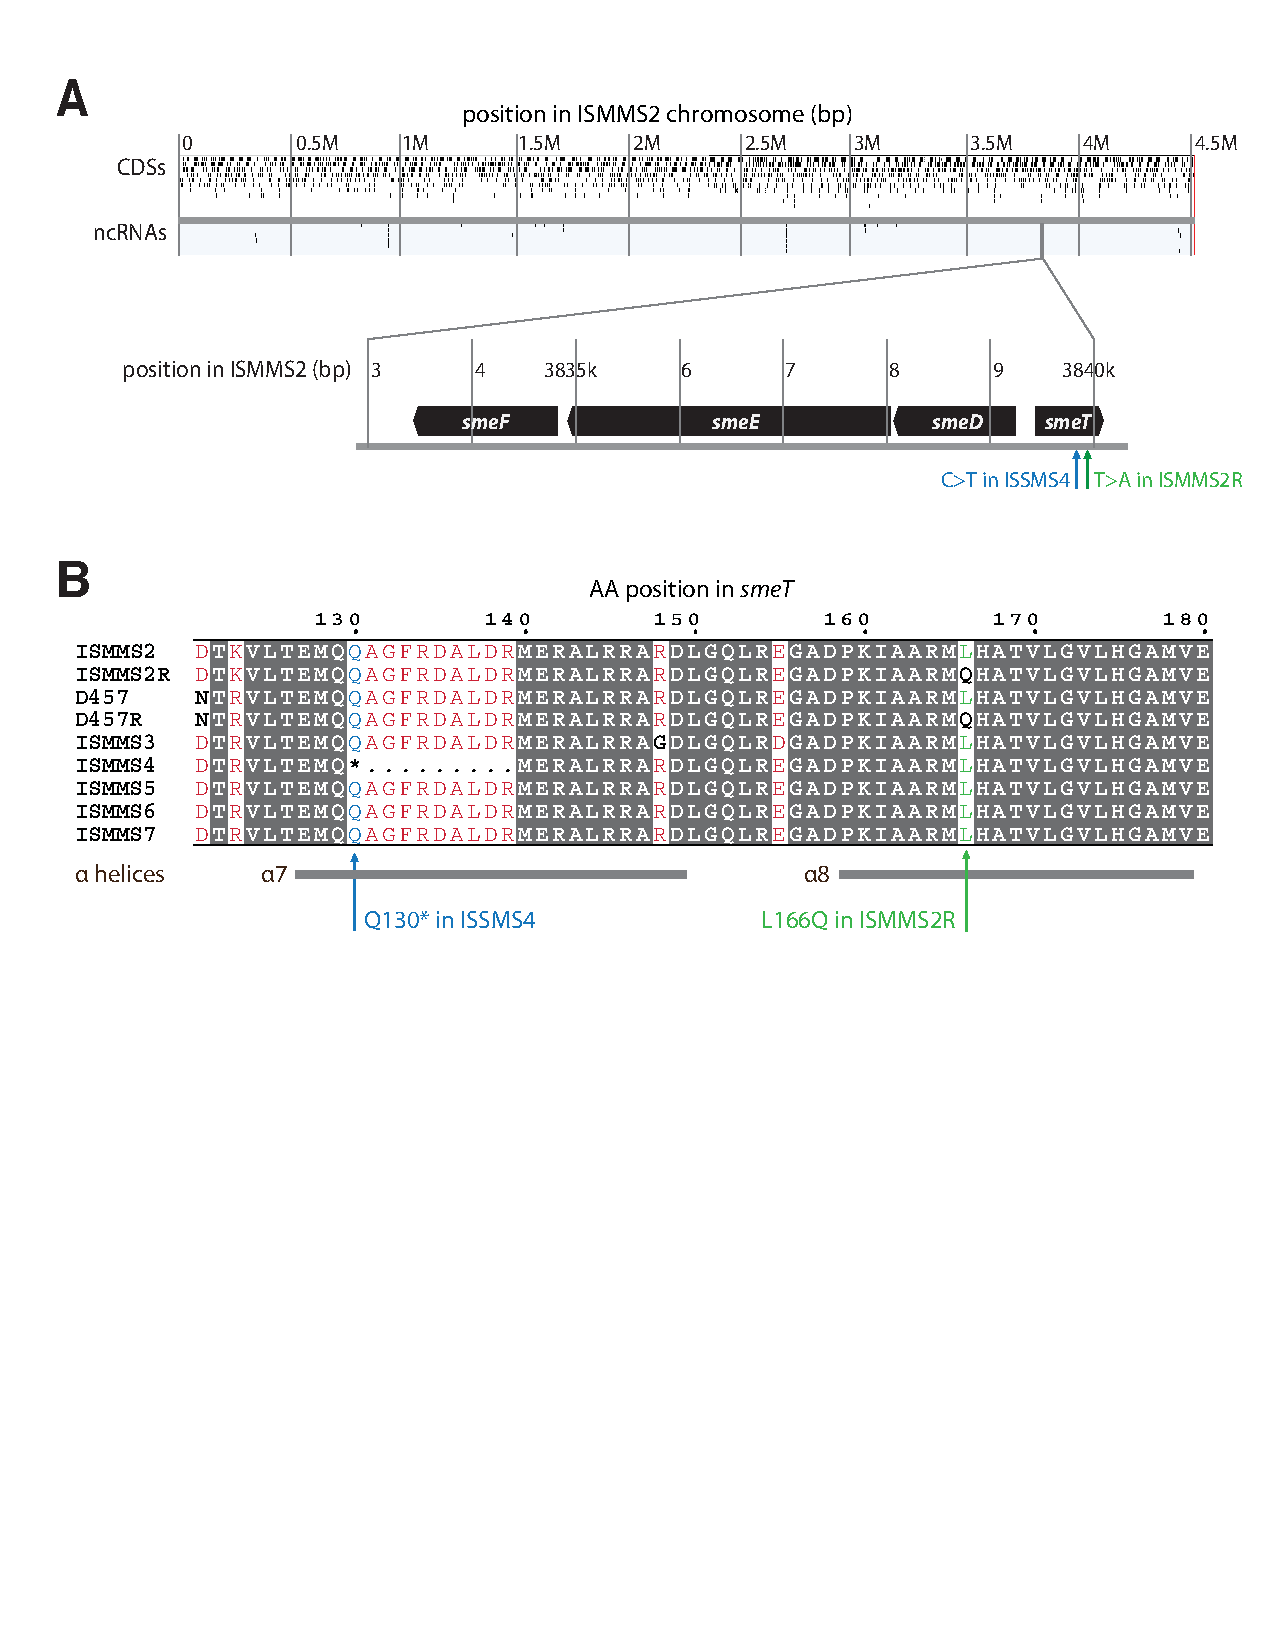
\includegraphics[width=\textwidth]{chap2/snp_location}
  \fullwidthlabelcaption{fig:snp_location}{SNVs observed in quinolone-resistant \emph{S. maltophilia} clinical isolates.}{
    \textbf{Single-nucleotide variants (SNVs) observed in quinolone-resistant \emph{S. maltophilia} clinical isolates.} A, assembled circular chromosome for ISMMS2, including predicted coding domain sequence (CDS) and noncoding RNA (ncRNA) features drawn with ChromoZoom. Horizontal position corresponds to base pair location. The \emph{smeDEF} operon is shown in the detail callout, which highlights both the \emph{smeT} c.497T>A SNV that emerged in ISMMS2R and the aligned location of the \emph{smeT} c.388C>T SNV (encoding a premature stop codon) in ISMMS4. ISMMS2 and ISMMS2R are serial isolates from a single patient before and after development of quinolone resistance, while ISMMS4 was quinolone-resistant at initial isolation from a different patient. B, multiple sequence alignment of part of the predicted \emph{smeT} product in each of the clinical isolates, the D457 reference assembly, and its quinolone resistant counterpart D457R. Predicted α-helices are labeled as grey bars below the sequence. Positions identical in all sequences are shaded with a dark gray background, equivalent substitutions are typeset in red, and non-equivalent substitutions are typeset in boldface black. The L166Q and Q130* (*, stop codon) polymorphisms are highlighted.
  }
\end{figure*}

The same nonsynonymous mutation has been previously observed in an in vitro strain of \emph{S. maltophilia}, D457R, created by selecting single-step tetracycline-resistant mutants from the antibiotic-susceptible clinical strain D457 \autocite{Alonso1997,Sanchez2002}. The mutation is in the eighth α-helix of the \emph{smeT} protein \autocite{Hernandez2009}, which homodimerizes to repress transcription of the \emph{smeDEF} operon \autocite{Hernandez2009,Sanchez2002}. Although the mutation is not in the DNA-binding region, it has been shown to disable the repressor activity of \emph{SmeT},\autocite{Sanchez2002} leading to upregulation of \emph{SmeDEF} and conferring an MDR phenotype \autocite{Alonso2001}.

Figure \ref{fig:snp_location}B shows an amino-acid sequence alignment comparing \emph{SmeT} in D457 and D457R to aligned sequences from our seven isolates. Notably, while none of the remaining isolates shared the same Leu-166→Gln (c.497A>T) mutation, another isolate resistant to levofloxacin, ISMMS4, displayed a C>T mutation at position 388 of \emph{smeT} that creates a premature stop codon that likely disrupts \emph{smeT} function (Figure \ref{fig:snp_location}A and \ref{fig:snp_location}B).

\begin{figure}[htb]
  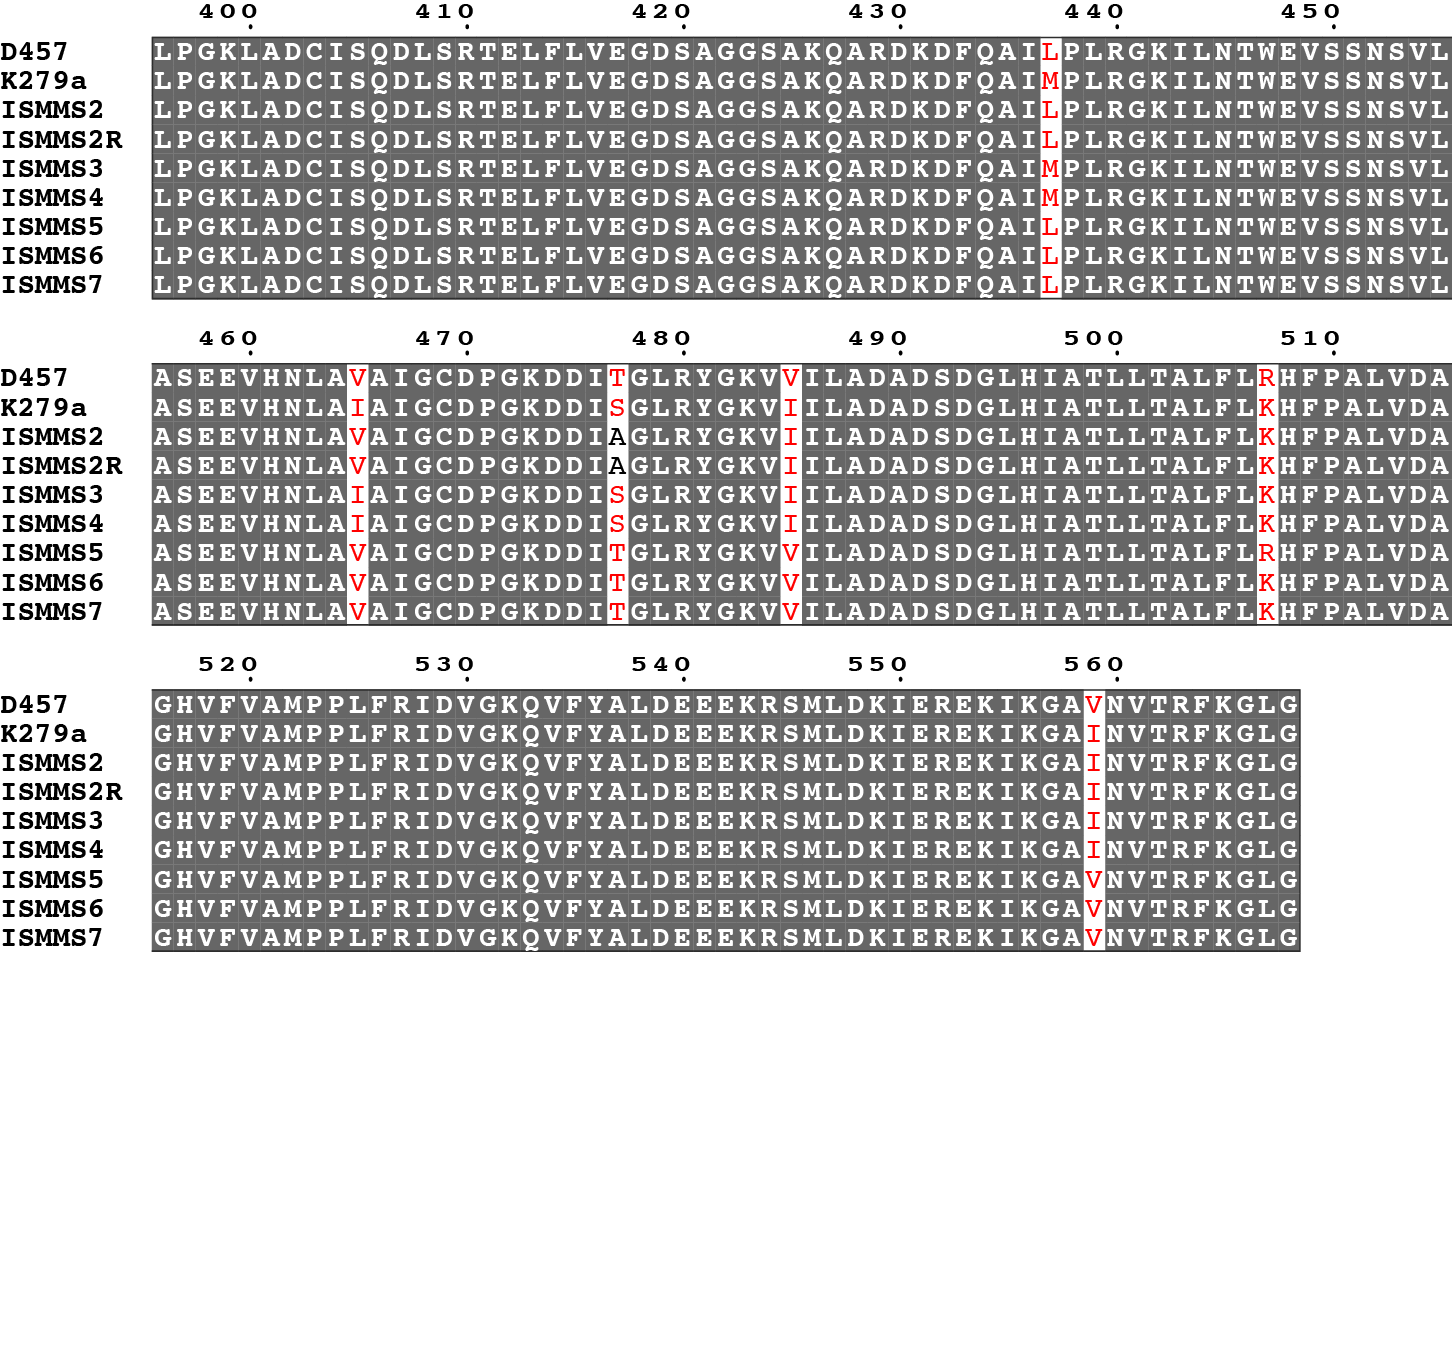
\includegraphics[width=\textwidth]{chap2/qrdr_locus}               
  \caption[Amino-acid sequence alignment for the quinolone-resistance determining region (QRDR) of the \emph{parE} gene]{Amino-acid sequence alignment for the quinolone-resistance determining region (QRDR) of the \emph{parE} gene for seven S. maltophilia clinical isolates (ISMMS2 through 7 and ISMMS2R) and two reference assemblies of clinical isolates obtained from GenBank.}
  \label{fig:qrdr_locus}
\end{figure}
 
The QRDR are loci within genes encoding topoisomerase II and IV subunits known for mutations that confer quinolone resistance in Gram-negative bacteria, although they appear to play a secondary role to efflux systems for resistance emerging during treatment of \emph{S. maltophilia} infection.\autocite{Valdezate2005} An amino-acid sequence alignment of the \emph{gyrA}, \emph{gyrB}, and \emph{parC} genes of our seven isolates and the reference clinical isolates D457 and K279a revealed no differences in the QRDR. Some variants were observed within the QRDR of \emph{parE} (Figure \ref{fig:qrdr_locus}), all of which were consistent with past observations in clinical isolates \autocite{Valdezate2002} except for an Ile-599→Val variant observed in three of our isolates and the D457 reference sequence.

\subsection{Diverse sources of \emph{S. maltophilia} identified with WGS}

Significant genomic diversity was observed among the \emph{S. maltophilia} isolates from all six patients. Figure \ref{fig:steno_phylo} shows a maximum-likelihood phylogeny with branch lengths scaled to SNV distances. Our isolates distribute widely among all four reference assemblies for complete \emph{S. maltophilia} genomes in GenBank. The distances of tens of thousands of SNVs seen in our phylogeny suggest that the natural diversity of pathogenic \emph{S. maltophilia} is greater than that captured by the current set of reference assemblies, even within a single hospital setting. 

\begin{figure}[htb]
  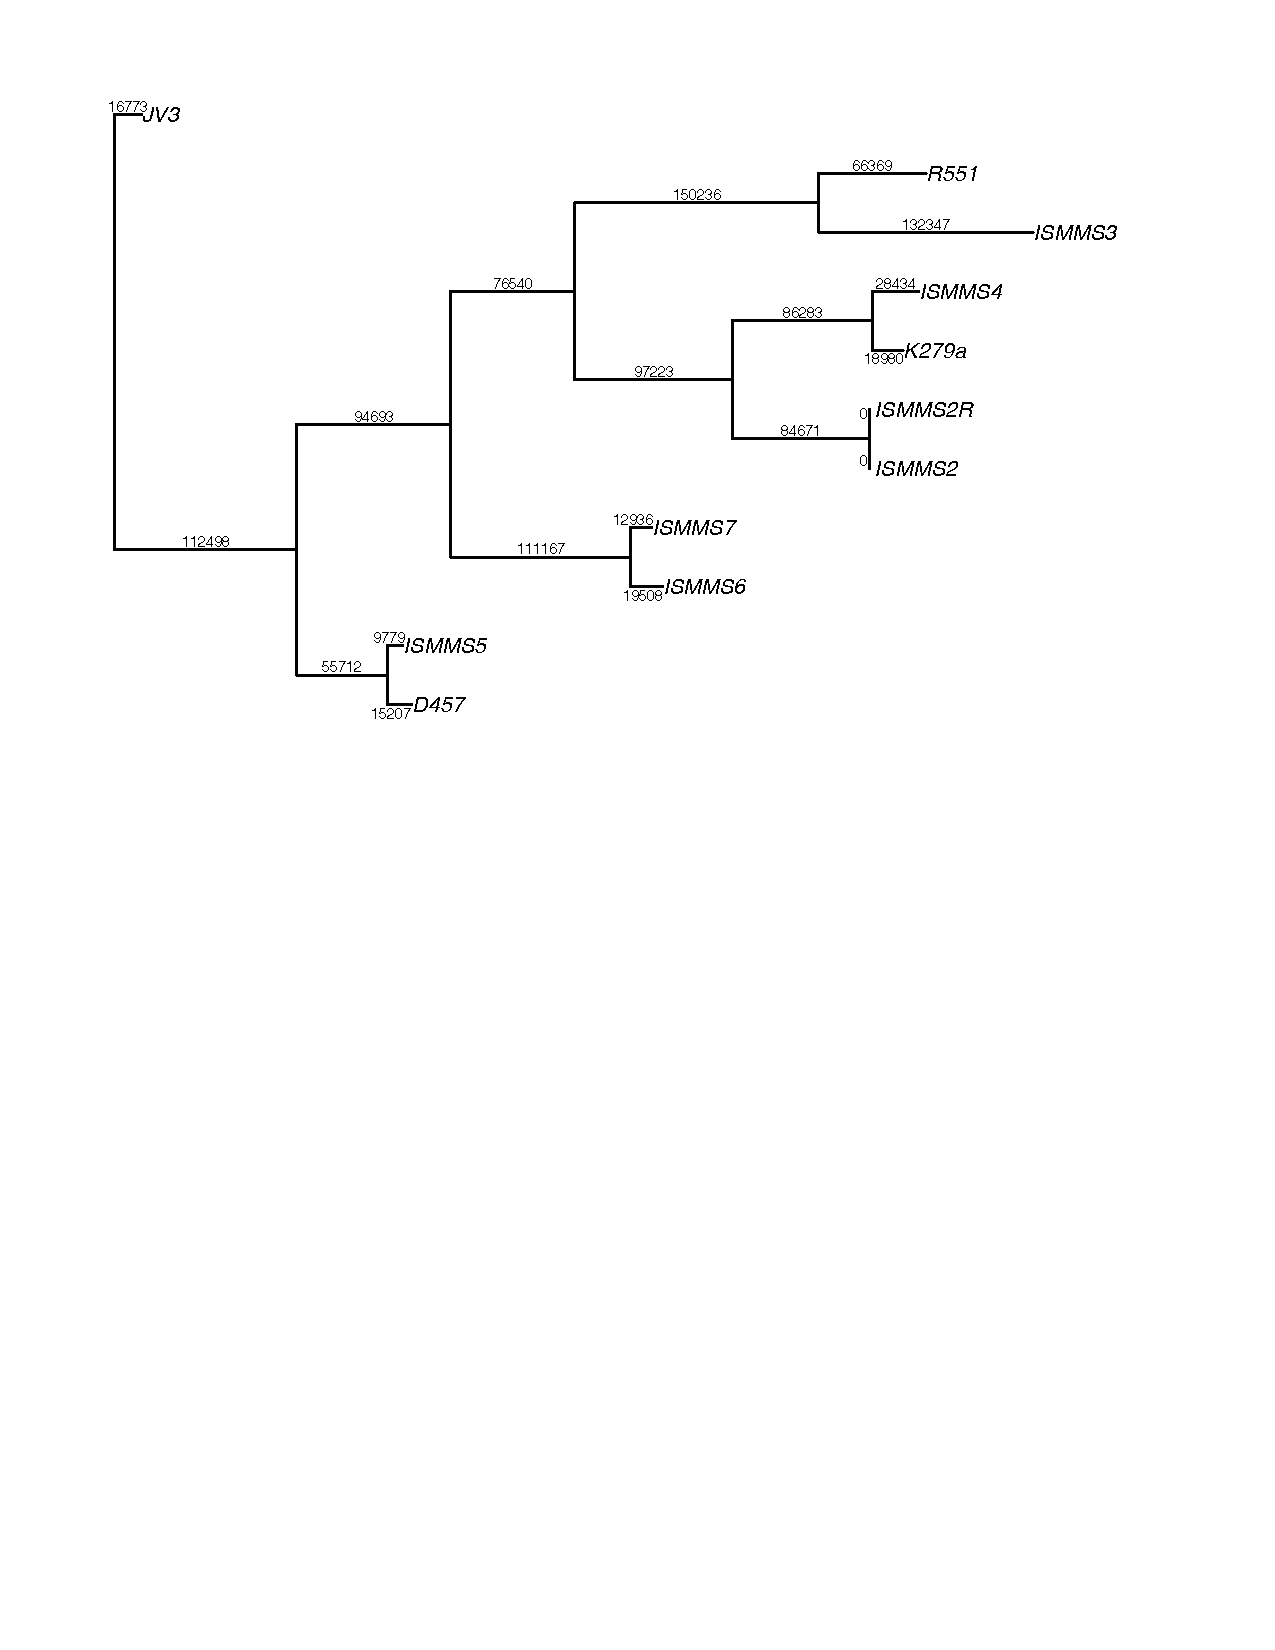
\includegraphics[width=\textwidth]{chap2/phylogram}               
  \caption[Phylogeny of seven \emph{S. maltophilia} clinical isolates]{Phylogeny of seven \emph{S. maltophilia} clinical isolates (ISMMS2 through 7 and ISMMS2R) and four reference assemblies obtained from GenBank. Trees were constructed by inferring ancestral states using RAxML-8.0.2; branch lengths correspond to single-nucleotide polymorphism (SNP) distances from branch points, and are drawn using R version 3.0.3 and the APE library version 3.1-1. The core genome did not contain the \emph{smeT} locus; therefore, the SNV differentiating ISSMS2 and ISMMSR is not observed in this tree.}
  \label{fig:steno_phylo}
\end{figure}

\begin{figure}[htb]
  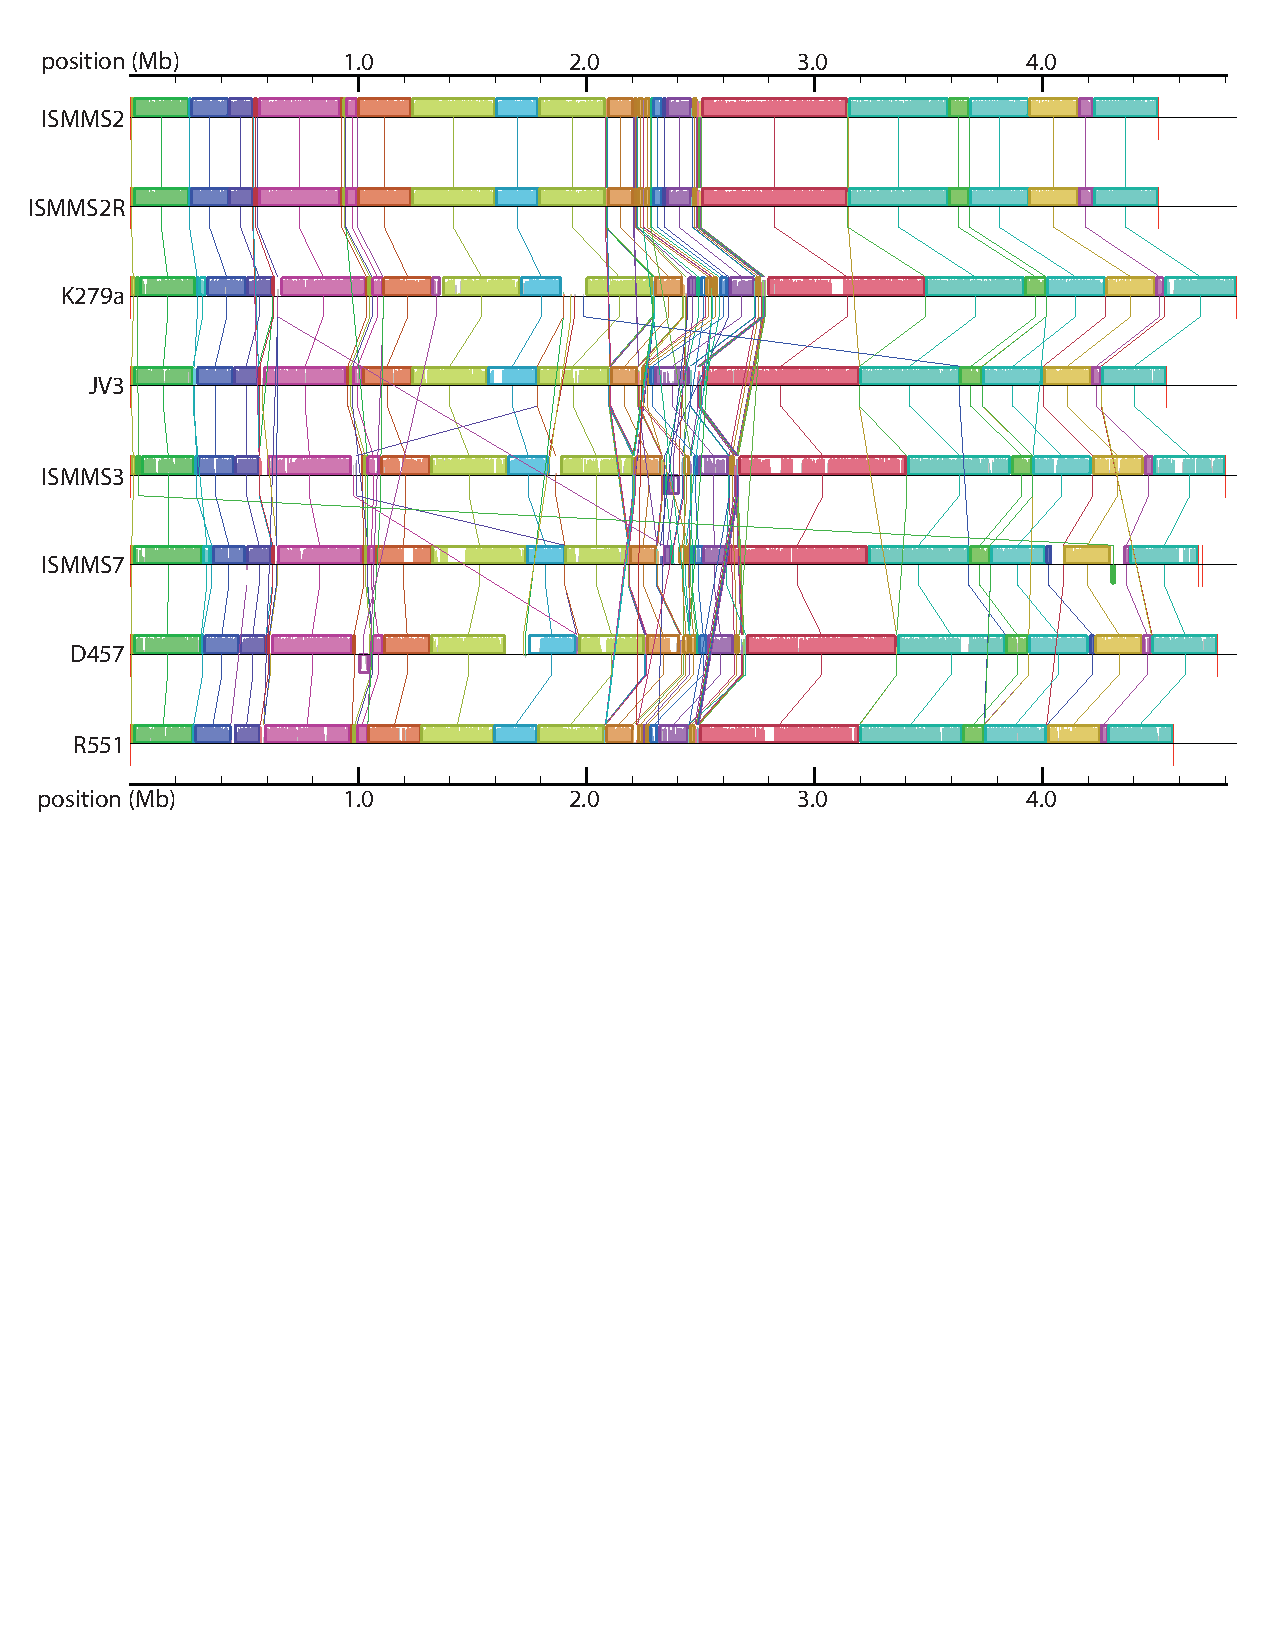
\includegraphics[width=\textwidth]{chap2/mauve_structural_variation}               
  \caption[Genome-scale comparison of four clinical isolates and four reference assemblies]{Genome-scale comparison of four fully assembled \emph{S. maltophilia} clinical isolates and four reference assemblies obtained from GenBank. Mauve 2.4.0 was used to plot locally collinear blocks (LCBs; conserved segments that appear to be internally free from genome rearrangements) as colored rectangles, with gaps representing non-homologous regions. Vertical bars inside each LCB rectangle show the average level of conservation at that region of the genomic sequence. Colored lines connect homologous LCBs among the genomes, and LCBs plotted below the centerline are in the reverse complement orientation relative to the ISMMS2 sequence. At top, sequences for the isolates from before and after development of quinolone resistance (ISSMS2 and ISSMS2R) in the case patient have identical structures.}
  \label{fig:mauve}
\end{figure}

Recombination is not an obvious source of diversity in our \emph{S. maltophilia} isolates. Figure \ref{fig:mauve} depicts whole genome alignments between the four clinical isolates where assembly produced a circularized chromosome and the four GenBank references, showing small areas of non-homology separating large regions of significant homology occurring generally in the same order for each genome. ISMMS2 and ISMMS2R are structurally identical, as expected for serial isolates, while recombination events among other strains are limited to small 1-2kb segments. Epigenetics motif analysis also suggests that the isolates are not related. Table \ref{tab:steno_epimotifs} shows different motifs in isolates from separate patients, implicating differences in type II \& III restriction modification systems between the isolates more likely to be caused by inter-strain/species horizontal transfer of methyltransferases than by intra-strain mutations.\autocite{Srikhanta2010} Together, this demonstrates that transmission did not occur among these six cases and that whole-genome sequencing can comprehensively capture genetic distances and structural variants among diverse clinical isolates of \emph{S. maltophilia}.

\begin{table}[ht]
  \centering
  \begin{tabular}{l l}
    \toprule
    Isolate name & Epigenetic motifs \\
    \midrule
    ISMMS2   & AGT\underline{A}CT \\
    ISMMS2R  & AGT\underline{A}CT \\
    ISMMS3   & None \\
    ISMMS4   & CAG\underline{A}G \\
    ISMMS5   & CTGG\underline{A}C, CACAN\underline{A}G \\
    ISMMS6   & CAAC\underline{A}C, CTG\underline{A}TG, CAACG\underline{A}C \\
    ISMMS7   & CAG\underline{A}G \\
    \bottomrule
  \end{tabular}
  \caption[Epigenetic motifs for clinical isolates of S. maltophilia]{Diverse epigenetic motifs, representing putative target sequences for each strain’s DNA methyltransferase enzymes, discovered for clinical isolates of \emph{S. maltophilia}.  Isolates are named as in Table \ref{tab:steno_pts}. The underlined A’s correspond to putative 6-methyladenine residues, which was the only modification type found in this study.}
  \label{tab:steno_epimotifs}
\end{table}

\section{Discussion}

This is the first report of WGS on serial isolates to characterize the emergence of a resistance mutation in \emph{S. maltophilia} during antibiotic treatment of an active infection. In contrast to studies sequencing highly resistant strains of \emph{S. maltophilia} to reveal various intrinsic and acquired antibiotic resistance genes,\autocite{Crossman2008,Zhao2015} where it remains difficult to assess their relative importance to the phenotype, performing WGS on serial isolates as resistance emerges in vivo allows the causative mutation(s) to be captured. In our patient, the mutation was a SNV that replicates a variant observed in an in vitro model strain created to study the MDR phenotype in 1997.\autocite{Alonso1997} Using WGS and susceptibility testing, we can confirm that this SNV was the only variant to emerge and that it was sufficient to confer quinolone resistance in a clinical case. This underscores the need for clinicians to consider repeating DST during monotherapy if clinical signs suggest therapy failure.

\emph{smeT} appears to play a central role in adaptive resistance to quinolones and other antibiotics effluxed by \emph{smeDEF}, like tetracycline, chloramphenicol, erythromycin, and aminoglycosides. Since any mutation that inactivates this protein would be able to derepress \emph{smeDEF} and confer resistance, \emph{smeT} is under intense selective pressure in the presence of these drugs. In this study, we observed not only a deleterious SNV in the strain that displayed resistance (ISMMS2R), but a premature stop codon in \emph{smeT} in a strain that was already resistant at first isolation (ISMMS4). Certain nucleotide positions appear to be under greater selective pressure than others, as evidenced by our observation of the same mutation that occurred in D457R, and a relative paucity of nonsynonymous coding mutations in \emph{smeT} observed among clinical \emph{smeT} isolates.\autocite{Sanchez2004} Since sustained overexpression of \emph{smeDEF} is physiologically unfavorable \autocite{Alonso2004}, it is possible that pathogenic strains of \emph{S. maltophilia} rely on natural diversity of mutations in the \emph{smeT} locus to activate or deactivate \emph{smeDEF} expression, allowing for rapid adaptation to antibiotic stress, though further study is needed.

Since resistance from a single SNV emerged during a short course of ciprofloxacin, clinicians should be cautioned about using quinolone monotherapy for \emph{S. maltophilia} bacteremia, as highlighted in recent retrospective studies.\autocite{Cho2014a,Wang2014} The wide variety of MDR phenotypes and unreliability of DST results has created uncertainty about appropriate treatment for \emph{S. maltophilia}, but SXT remains the most common choice for monotherapy.\autocite{Brooke2012,Cho2014a,Wang2014} SXT resistance in \emph{S. maltophilia} is not known to be caused by efflux systems but has been linked to Class 1 integrons and ISCR elements.\autocite{Brooke2012} This suggests that spontaneous resistance is less likely to emerge with SXT monotherapy, although a clinical trial comparing the two antibiotics is warranted.\autocite{Cho2014a,Wang2014}

In conclusion, characterizing the full extent of genetic alterations that \emph{S. maltophilia} utilizes to develop antibiotic resistance in vivo and improving genomic surveillance of clinical strains will help refine antibiotic selection criteria available to clinicians. This study furthermore highlights the utility of WGS for profiling the precise mutations underlying emerging antibiotic resistance in clinical cases of bacteremia.

\section*{Notes}

A shortened version of this chapter was published in \textit{Antimicrobial Agents and Chemotherapy}.\autocite{Pak2015a}

\subsection{Funding}

Funding was provided by the Icahn Institute for Genomics and Multiscale Biology at Mount Sinai, and also in part by the NIAID-supported NRSA Institutional Research Training Grant (5 T32 AI 7647-13) for Global Health Research (DRA).

\subsection{Conflict of Interest}

The authors have no conflicts of interest to disclose.

\subsection{Acknowledgements}

We thank Timothy O’Donnell, Tavi Nathanson, Jose Clemente, Flora Samaroo, Angelo Rendo, and members of the clinical microbiology laboratory at Mount Sinai for their contributions. This work was supported in part by the resources and expertise of the Department of Scientific Computing at the Icahn School of Medicine at Mount Sinai.